\author{Paul Hoffmann}
\graphicspath{ {./src/chapters/developer/media/} }

\chapter{Important Frontend Components}
\section{React Components}
The frontend is splitter in multiple React components. First of all
there are the Website is splatted in Footer App and Header. Header
and Footer are called from the App component\\
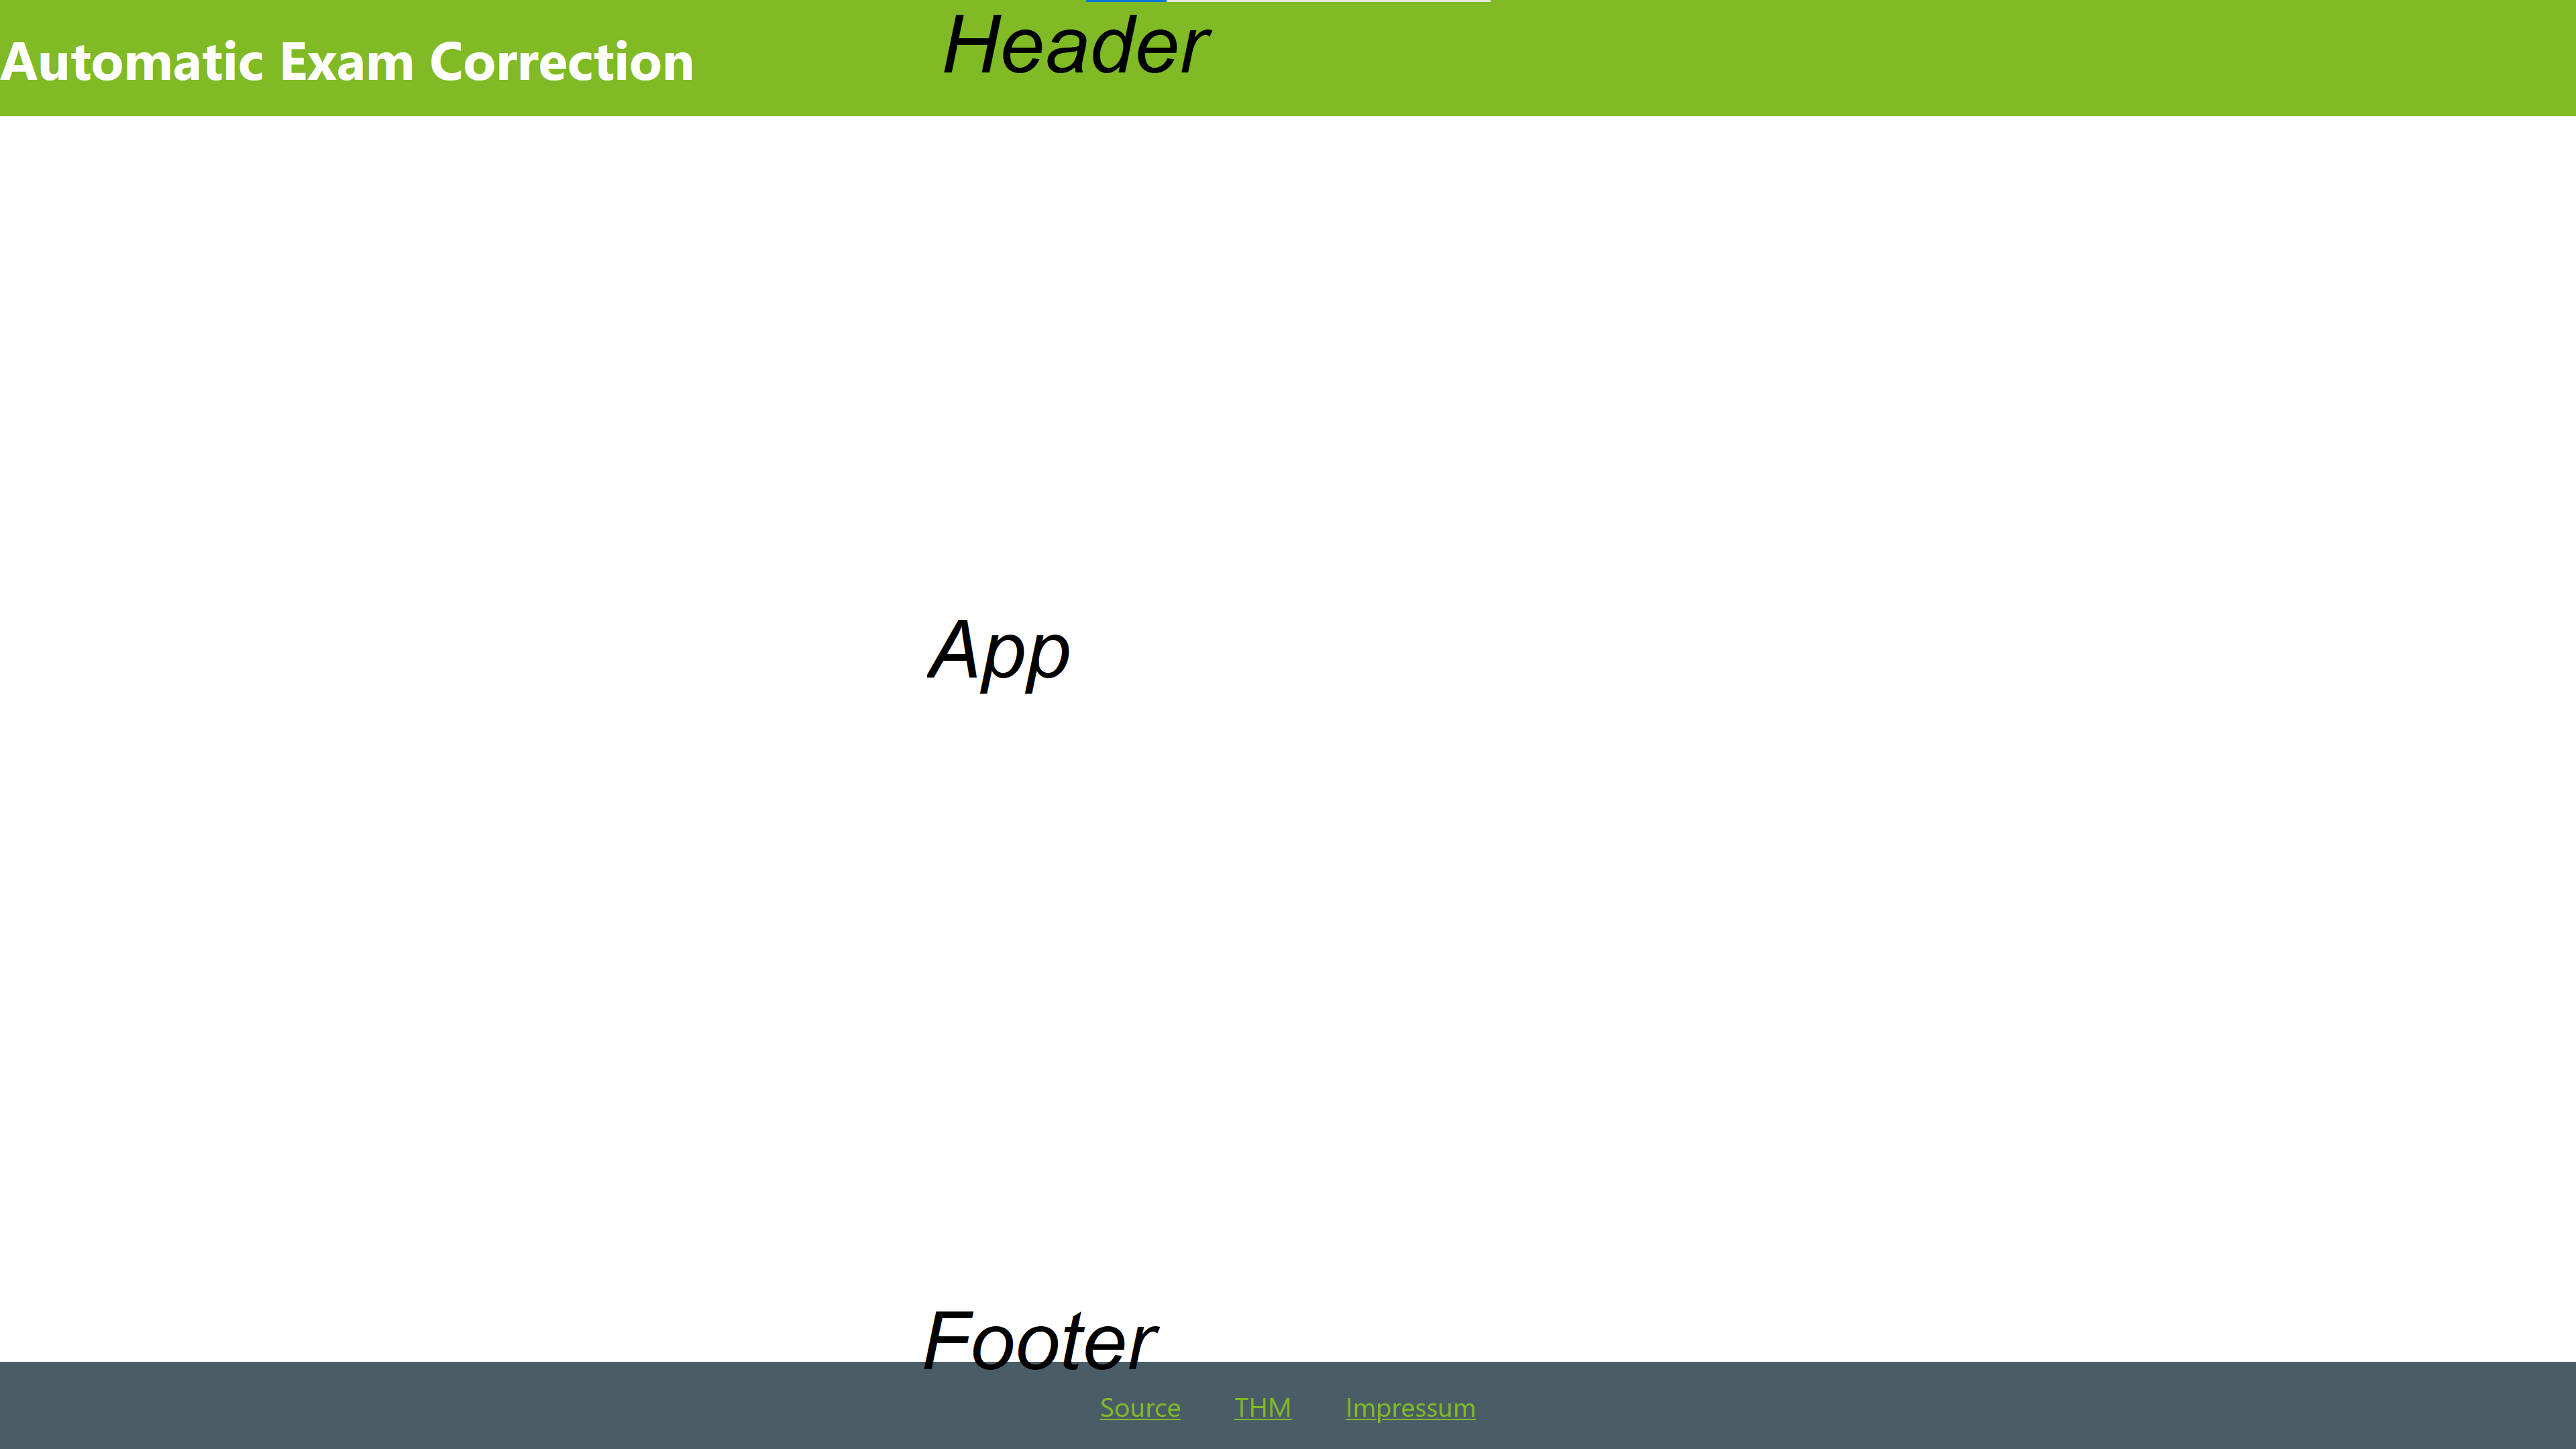
\includegraphics[width=\textwidth]{app}
The App renders 3 different views: TaskSelector, ReviewOverview,
ReviewExam. 
The App contains the "ExamContainer" the main State for the whole
Application

\section{TaskSelector Component}
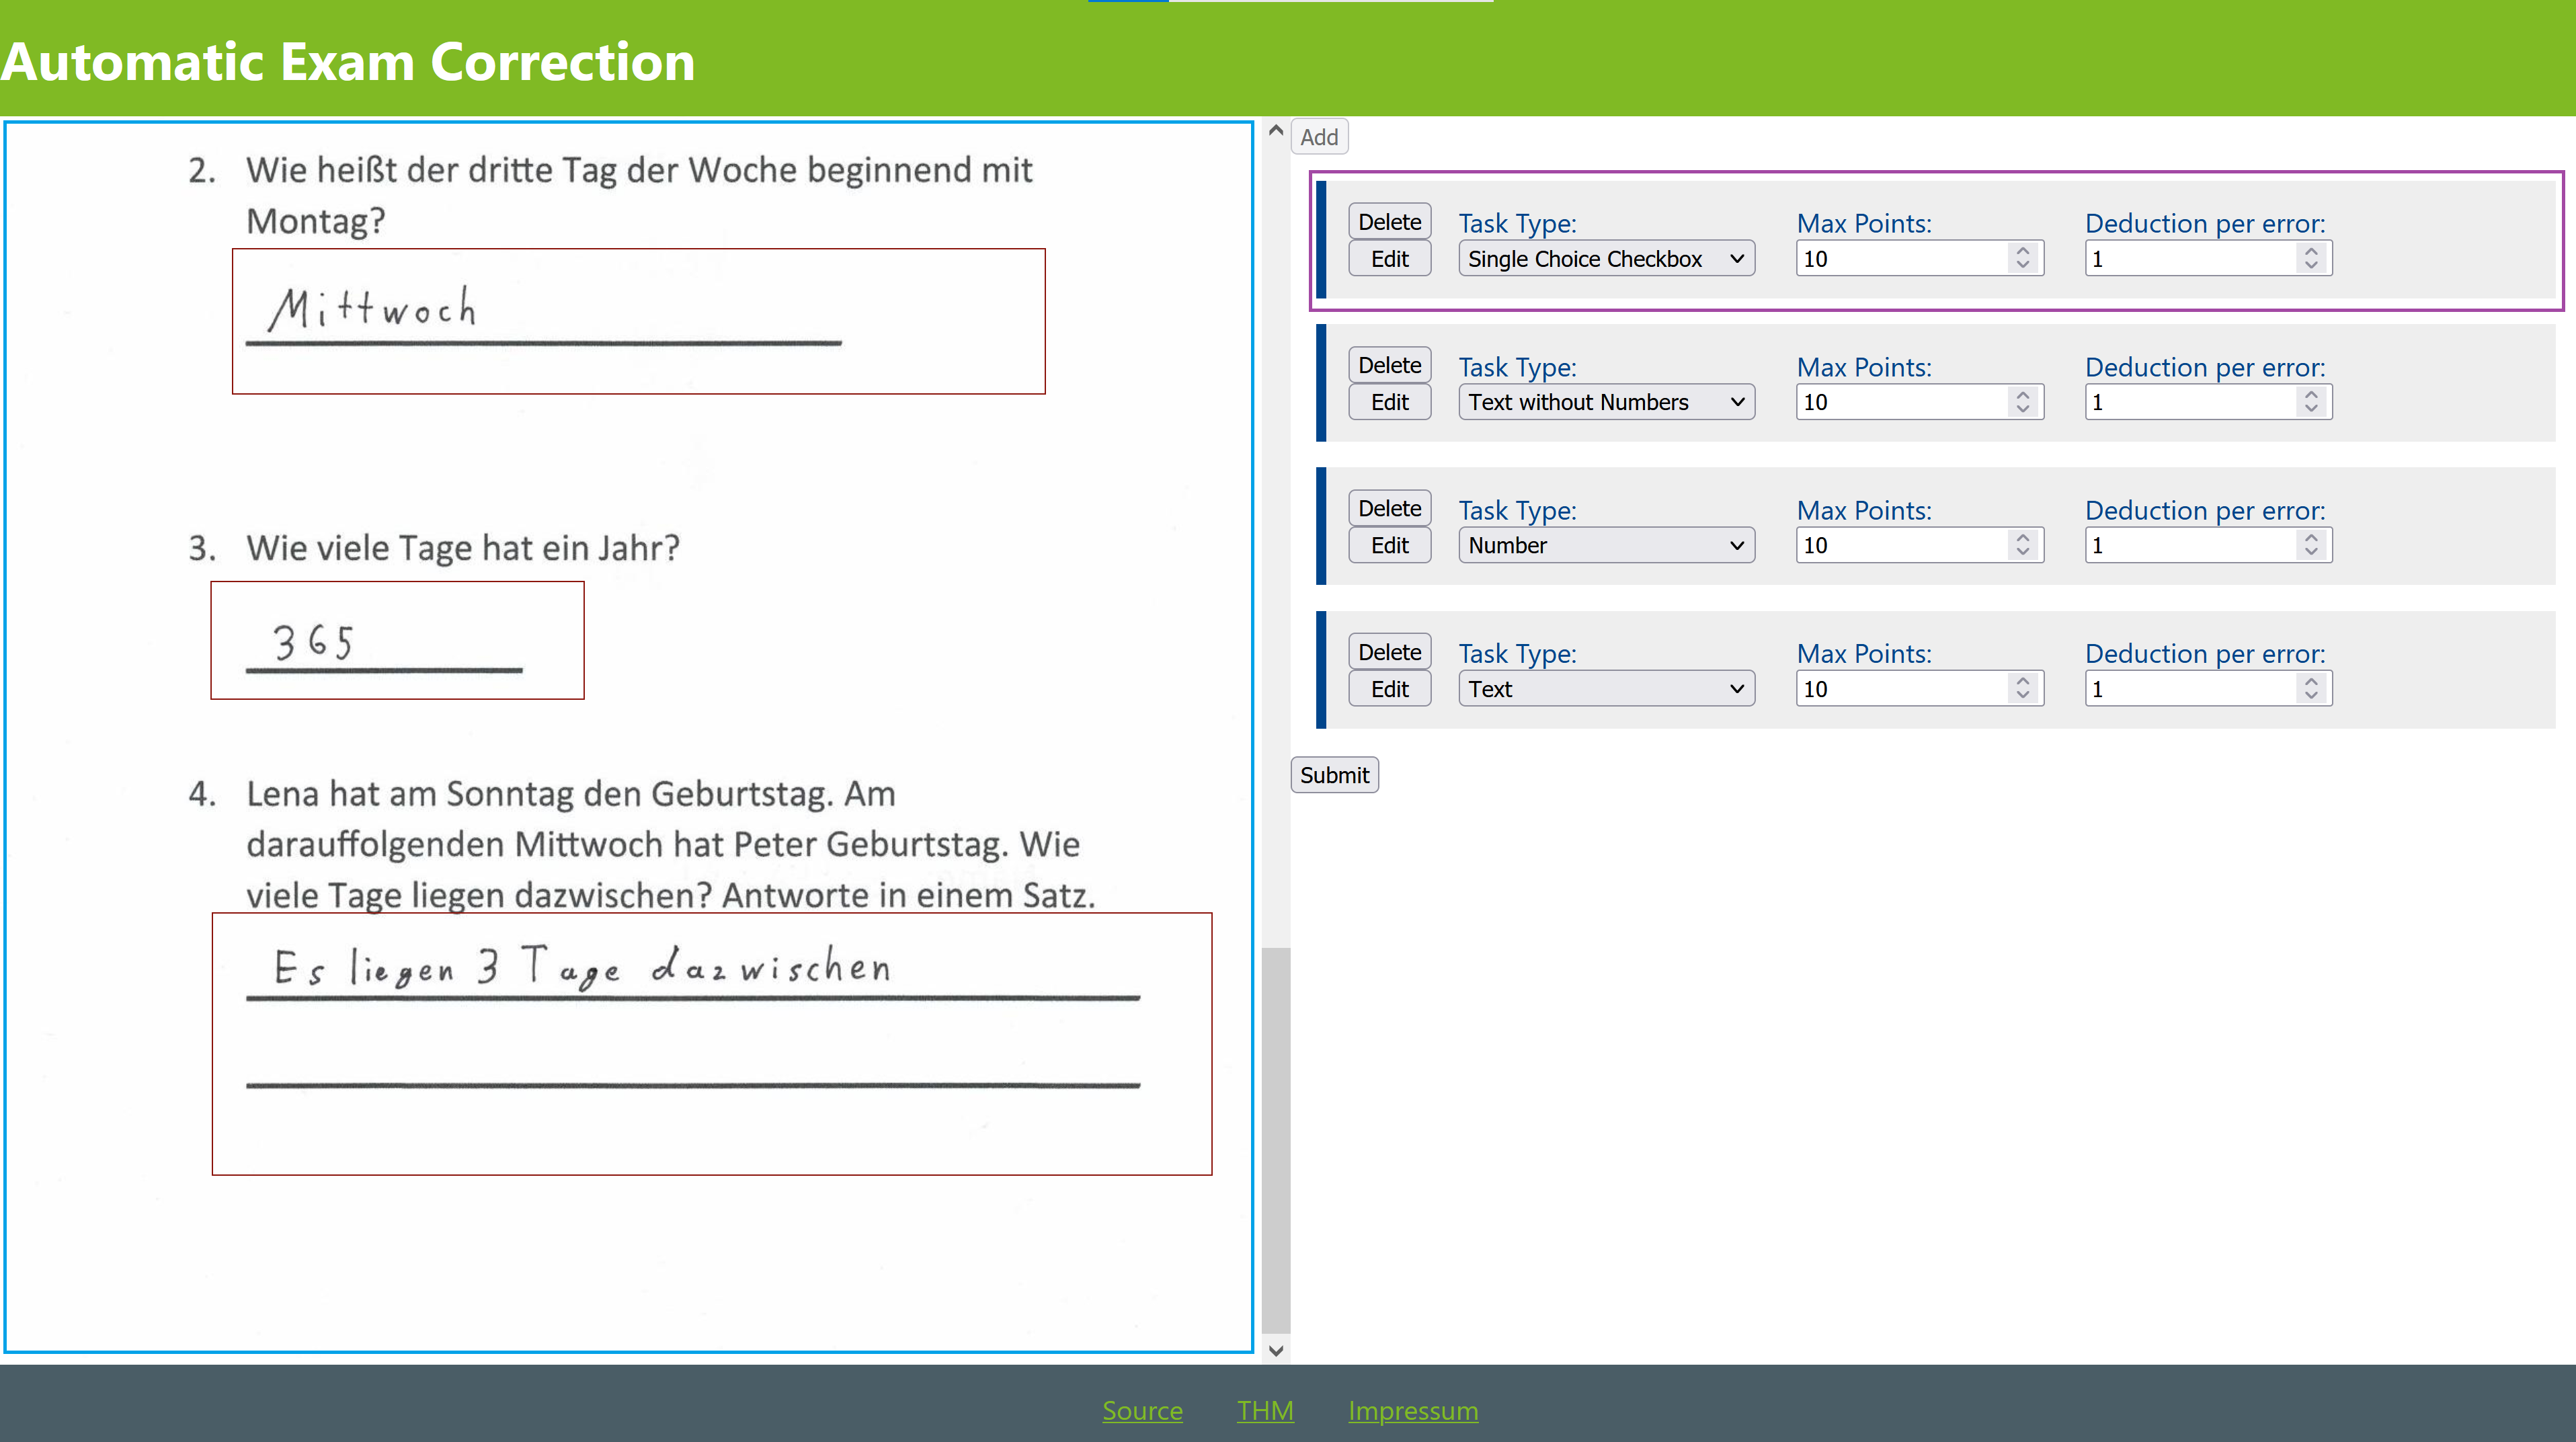
\includegraphics[width=\textwidth]{taskselector}
The TaskSelector is splatted in a left and a right column.

Props\\
\begin{tabularx}{\textwidth}{|l|X|} 
\hline
exam & The exam that should be viewed. Called only with
eamContainer.correctExam \\
\hline
setExam & setter for exam \\
\hline
examContainer & the whole examContainer state live at App\\
\hline
setExamContainer & setter for examContainer \\
\hline
setStudentExams & setter for examContainer.studentExams \\
\hline
leave & a function for leaving the examContainer and moving on in
the Process. It changes a state in App \\
\hline

\end{tabularx}

\subsection{Image Selection}
When a user selects an Image it gets loaded and saved as base64
string in ExamContainer.correctExam.image .
When a user selects a Pdf it gets send to the backend where it gets
converted to png. Afterwards it gets saved as base64 string in
ExamContainer.correctExam.image . 

\subsection{CroppingArea}
Marked blue\\
The image in the Cropping are is exam.image. The Cropping area uses
a component called Cropper which is just a wrapper around ReactCrop
from the library react-image-crop.

\subsection{Rectangle Component}
For every Task in examcontainer.correctExam.tasks there is a
Rectangle components, with x, y, width and height. It is just a div
with css styling set so it has a red border and appears on the tasks
selection.\\
Important: In a Task x, y, width, height are stored as integers and
are relative to to original image. Rectangle expects values relative
to the cropping area. This happens through a conversion.

\subsection{Add Button}
The Add takes the current crop from the croppingArea and creates a
new Task in exam.tasks .

\subsection{TaskEditingAreas Component}
For each Task there is a TaskEditingArea.

\subsection{TaskEditingArea Component}
Marked purple\\

Props\\
\begin{tabularx}{\textwidth}{|l|X|} 
\hline
task & The Task to display \\
\hline
taskId & important for the key \\
\hline
setTask & setter for task \\
\hline
loadCroppingArea & Gets called when editing the task area \\
\hline
deleteTask & delete this task from exam.tasks \\
\hline
saveCropInTask & Gets called when editing the task area \\
\hline
editing & is set when one Task is edited, so that the others are not
availible for editing\\
\hline
setEditing & setter for editing \\
\hline
canEditAnswer & true when reviewing the answers from the backend \\
\hline
onHover & called when hovering over \\
\hline
onHoverLeave & called when stop hovering \\
\hline
\end{tabularx}

\section{ReviewOverview Component}
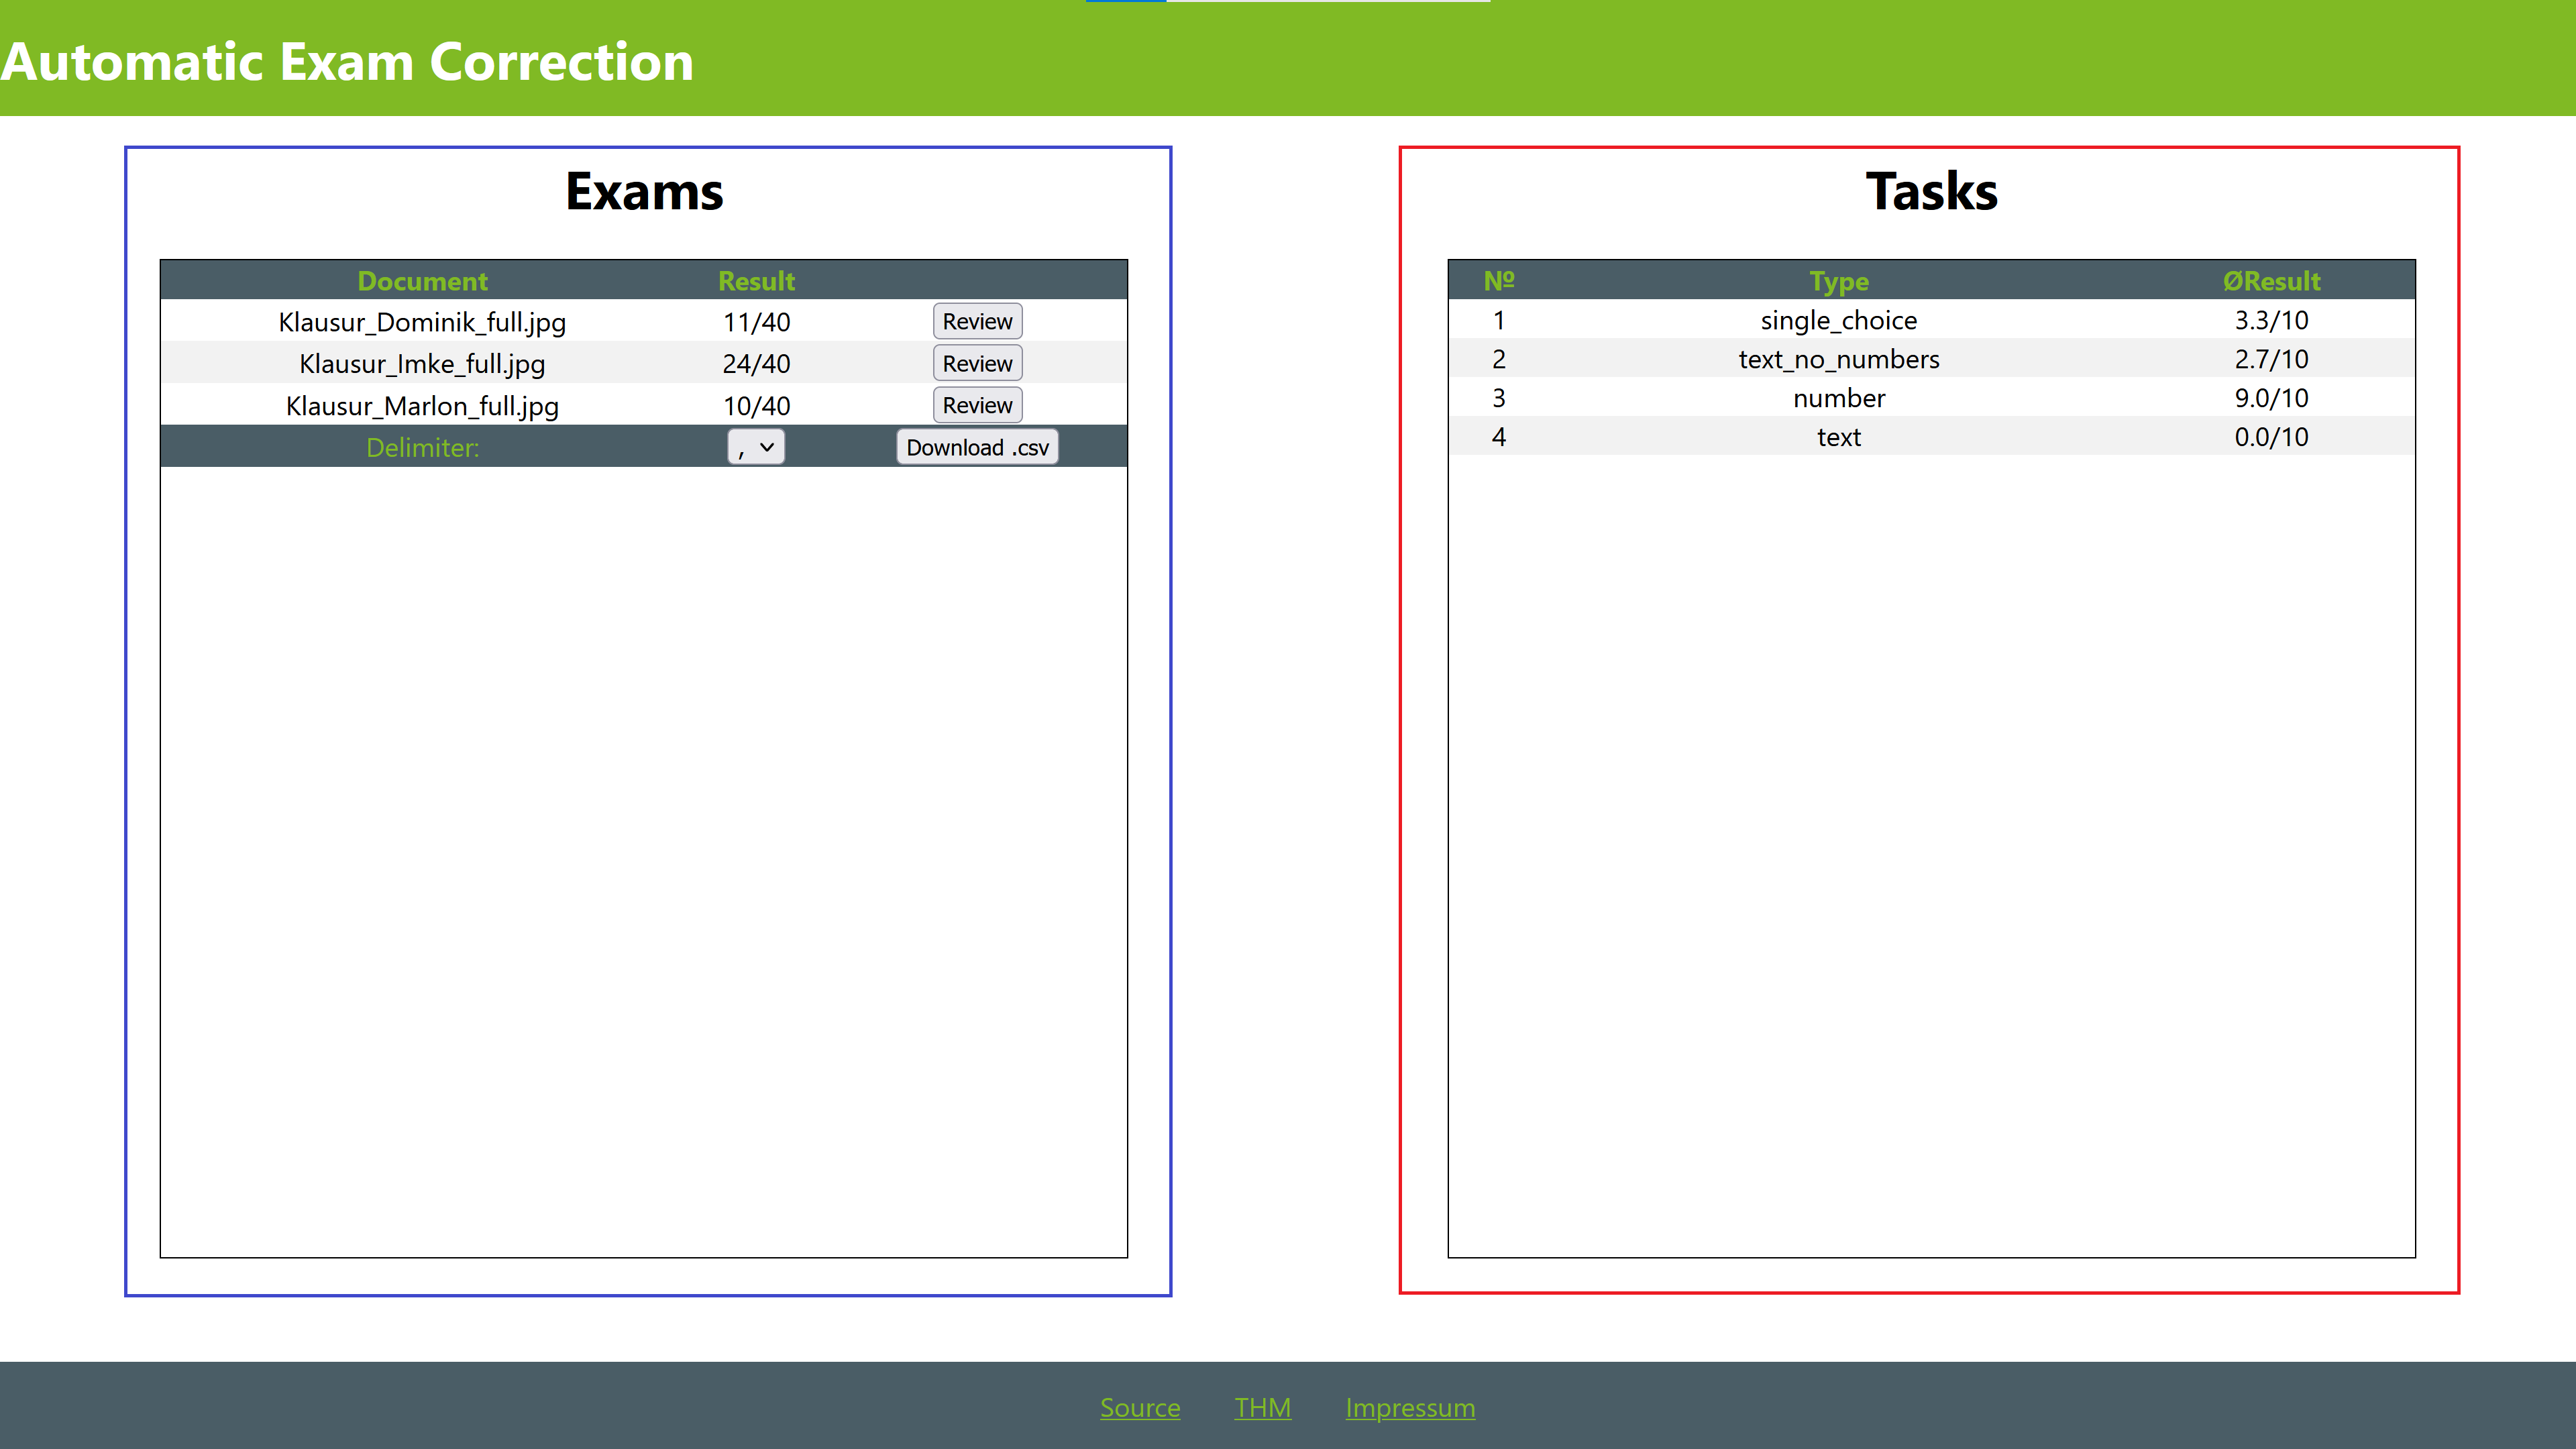
\includegraphics[width=\textwidth]{reviewoverview}
Props\\
\begin{tabularx}{\textwidth}{|l|X|} 
\hline
examContainer & examContainer state from App \\
\hline
reviewExam & review a given Exam \\
\hline
\end{tabularx}
\subsection{Exams Table(marked blue)}
Shows filename, an overview over the points they got and a button to
review the document.
Add the button you can download the table as csv. The delimiter is
imported, especially when using Exel. Exel reads different delimiter
depending of the system language. 
\subsection{Tasks Table(marked red)}
Shows a overview over the different Tasks.

\section{ReviewExam Component}
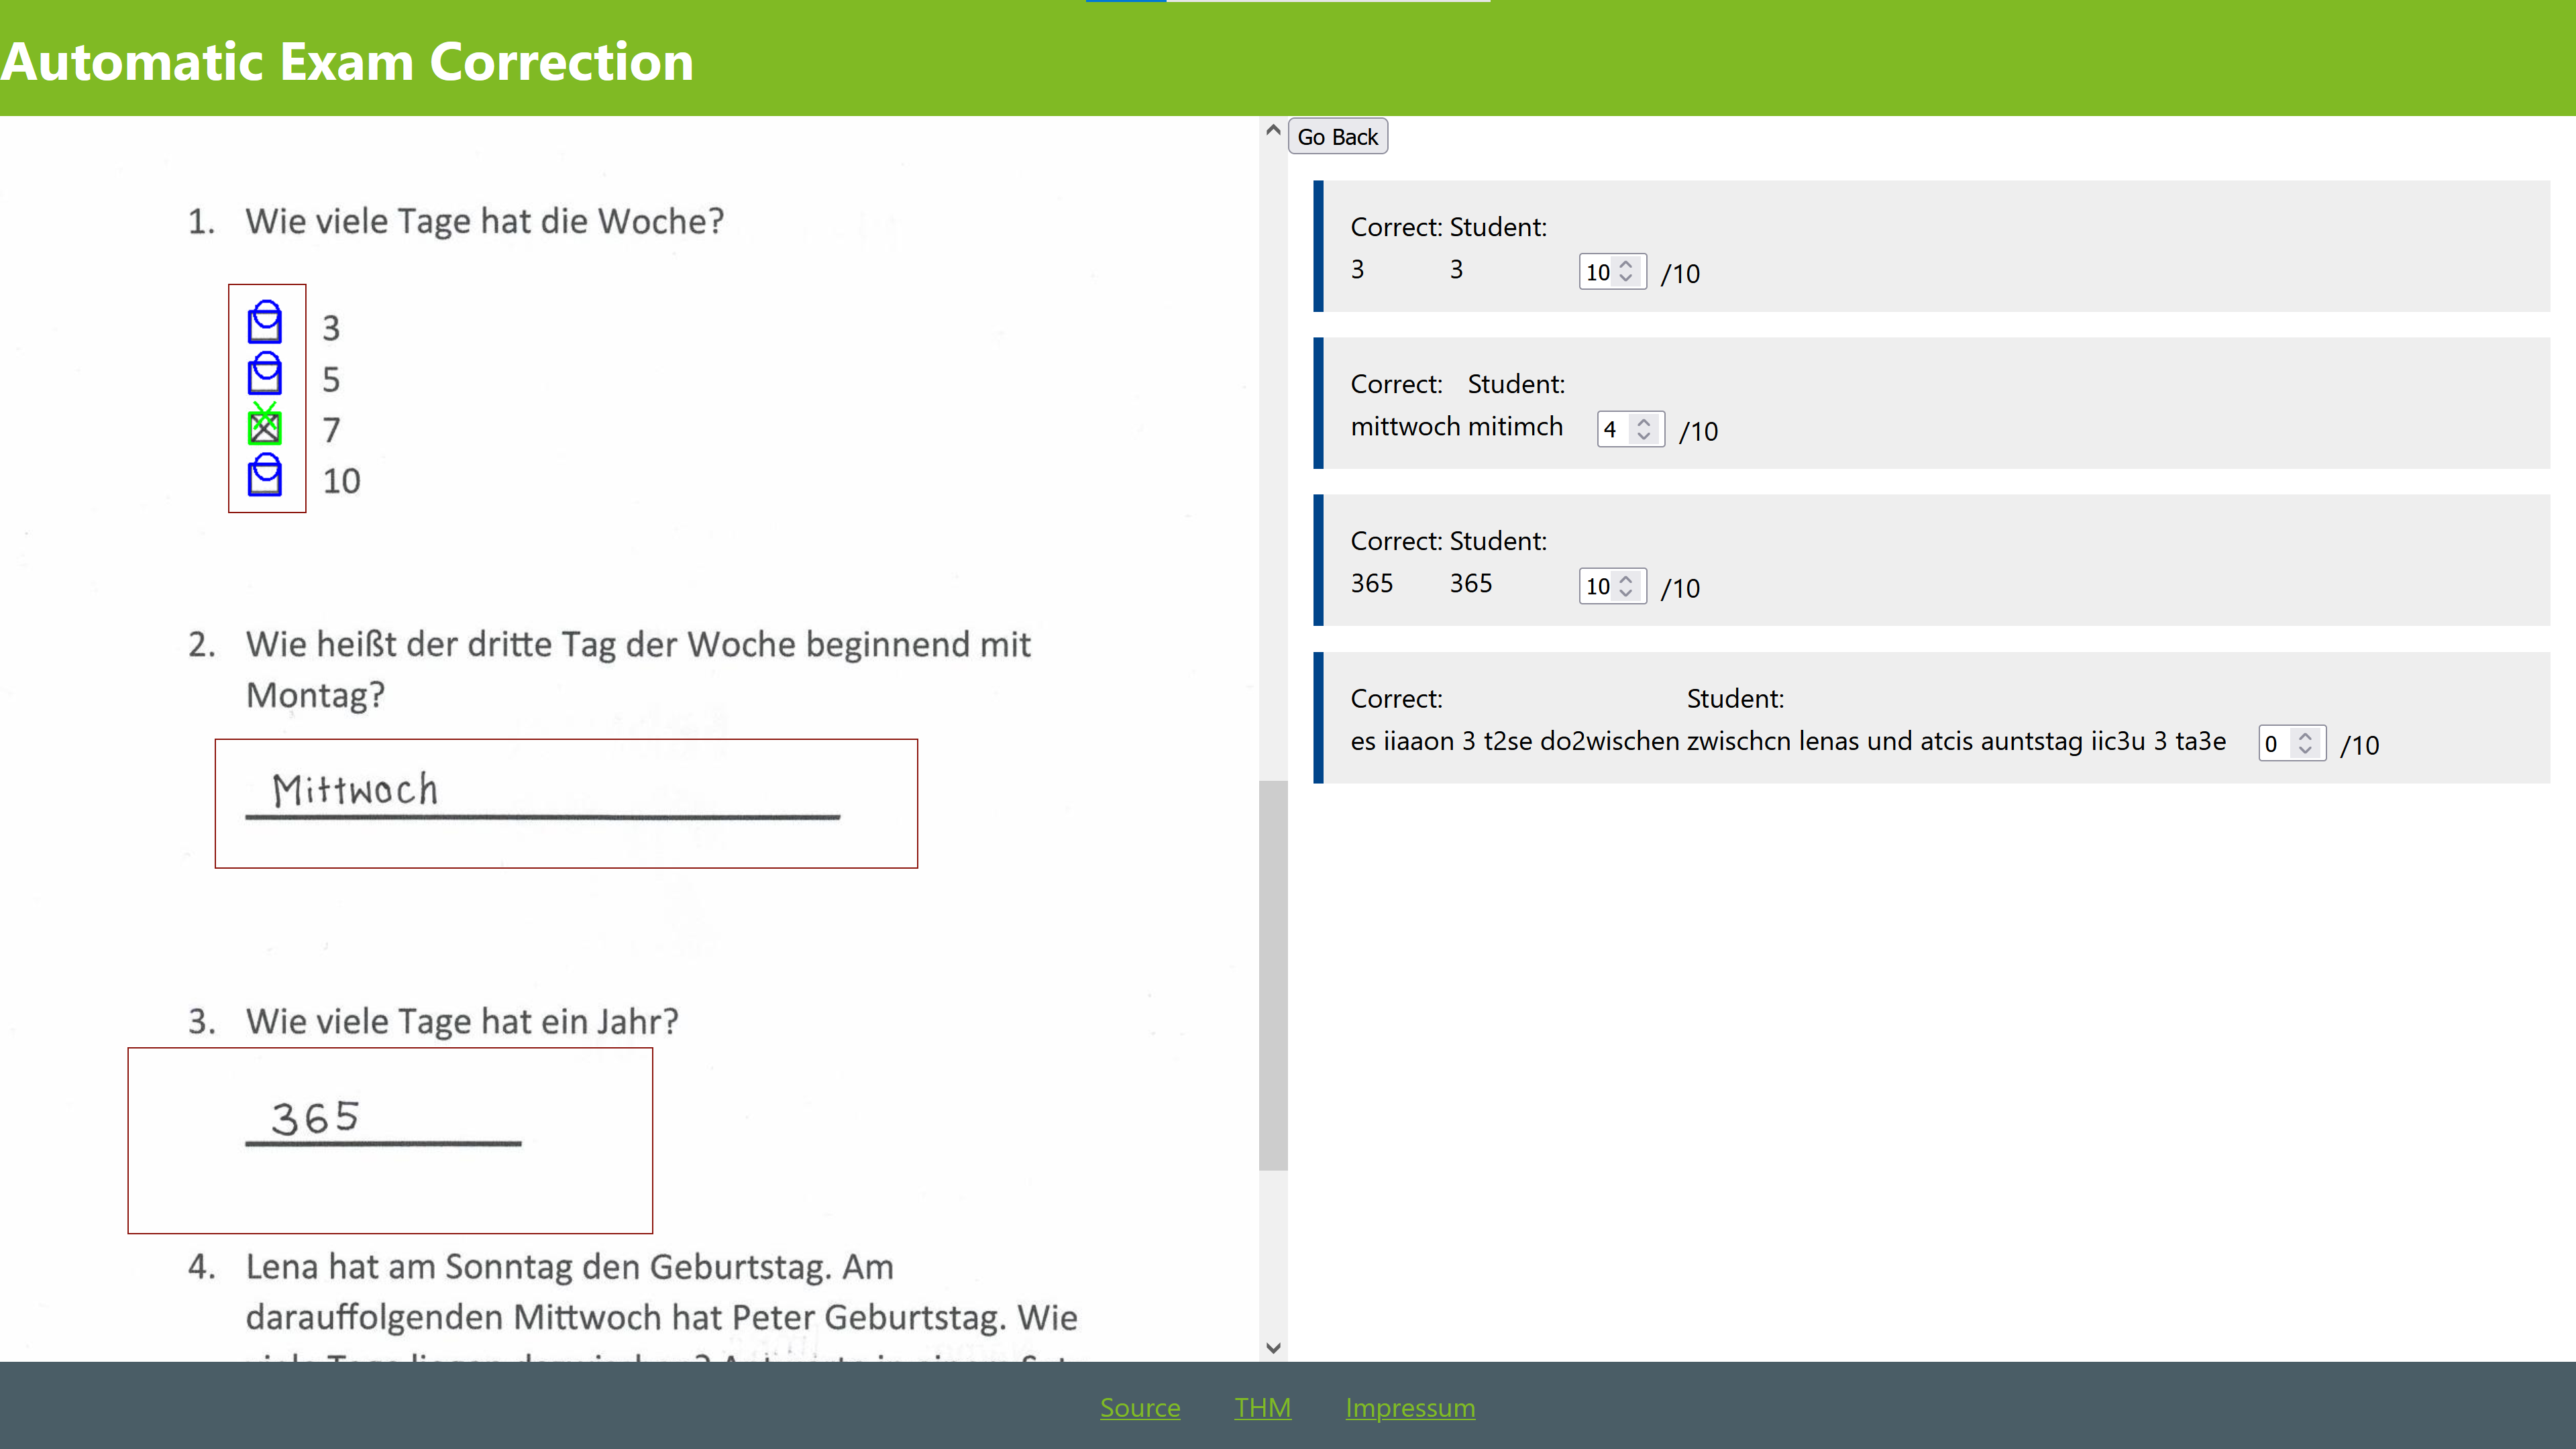
\includegraphics[width=\textwidth]{reviewexam}
This nearly the same as TaskSelector. The main differents is that
you obviously can not add new Tasks. The Areas right are called
TaskReviewingArea. Everything is nearly the same.



